En esta sección vamos a demostrar el potencial de la herramienta con algunos ejemplos de su funcionamiento. Validando el funcionamiento de ésta, y sus mejoras funcionales con respecto a la versión de Scratch4Robots de la que partimos.\\

Además de los ejemplos mostrados en este apartado, se ha creado una batería de pruebas con las que ver un ejemplo de funcionamiento de cada uno de nuestros bloques. Estas pruebas son proyectos Scratch, que el usuario puede cargar en el entorno de Scratch y usar como punto de partida para sus próximos proyectos.

\section{Evitar obstáculos con Kobuki}
\label{sec:evitar-obstaculos}

En este ejemplo hacemos uso de un robot con ruedas, para ser más exactos de un Kobuki. Para ejecutar las pruebas utilizamos Gazebo como entorno simulado, cargando un entorno con obstáculos repartidos.\\

El objetivo directo de este experimento es la programación de un robot, capaz de evitar obstáculos de forma autónoma, con la ayuda de un sensor láser incorporado en su parte frontal. Esto lo vamos a conseguir usando únicamente la lógica de la que disponemos en Scratch junto con la extensión que aporta nuestra aplicación Scratch4Robots.\\

Este ejemplo podemos verlo en la vida cotidiana día a día con las famosas aspiradoras autónomas (iRobot Roomba), por lo que vemos una aplicación directa que podría tener nuestra aplicación fuera del ámbito didáctico.\\

Vamos a seguir el ciclo de vida de nuestra aplicación, explicando el proceso que lleva a la consecución de nuestro objetivo.\\

En primer lugar y con ayuda de nuestros bloques, desarrollamos la aplicación en Scratch.\\

Una vez tenemos nuestro proyecto acabado y guardado, con la herramienta Scratch4Robots, ya instalada en nuestro equipo y mediante el uso de un solo comando realizaremos la traducción del proyecto. Esta simpleza en la ejecución la conseguimos mediante las funcionalidades que nos aporta ROS para la ejecución de nodos, esto se consigue tras la labor de integración realizada. El comando a ejecutar sería:\\
\begin{lstlisting}[language=json,firstnumber=1]
~$ rosrun scratch4robots scratch2python myapplication.sb2
\end{lstlisting}

Explicando un poco el comando anterior, \textit{ROSRUN} sería el comando que nos aporta ROS, capaz de ejecutar nodos de un paquete ROS, \textit{scratch4robots} es nuestro paquete ya instalado en la máquina, \textit{scratch2python} sería el nodo interno de nuestra aplicación encargada de la traducción a Python y por último se añado el proyecto Scratch que queremos traducir.\\

Tras la traducción obtenemos un nodo ROS completamente preparado para su ejecución sobre el robot simulado, únicamente con la dependencias de un fichero de configuración que describiremos a continuación:\\

\begin{lstlisting}[language=json,firstnumber=1]
robot:
  Motors:
    Server: 2 # ROS
    Topic: "/mobile_base/commands/velocity"
    Name: robotMotors
    maxW: 0.7
    maxV: 4

  Laser:
    Server: 2 # ROS
    Topic: "/scan"
    Name: robotLaser

  Pose3D:
    Server: 2 # ROS
    Topic: "/odom"
    Name: robotPose3d

  Camera1:
    Server: 2 # ROS
    Format: RGB8
    Topic: "/cameraL/image_raw"
    Name: robotCamera1

  NodeName: robot
\end{lstlisting}

En este fichero se observa los distintos actuadores y sensores que necesitará nuestro nodo, además por cada sensor se define el Tópico al que nuestro nodo se subscribe para enviar y recoger los datos que necesitemos de nuestro robot. En este caso darle especial importancia a la obtención de los datos del sensor laser.\\

Con todo esto preparado solo faltaría ejecutar nuestro nodo sobre la simulación para ver los resultados.\\

\begin{figure}[H]
    \centering
    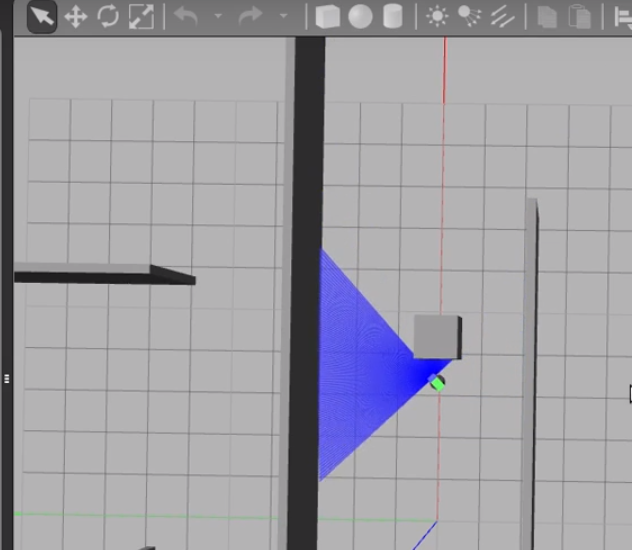
\includegraphics[scale=0.75]{img/robot-example.PNG}
  	\caption{Ejecución del nodo sobre el Kuboki}
  	\label{fig:curiosity}
\end{figure}


De esta forma, en pocos y sencillos pasos conseguimos programar un robot de forma autónoma para que evite cualquier obstáculo que se encuentre en su camino.


\section{Persecución entre drones}
\label{sec:persecucion-drones}

En este ejemplo por el contrario, como robot final utilizamos un dron, mucho más interesante desde el punto de vista práctico, aunque igual de interesante desde el punto de vista didáctico. Al igual que con la prueba anterior hemos utilizado Gazebo como motor de simulación.\\

El ciclo de vida es el mismo que el que hemos seguido para la ejecución del robot.

Primero se genera el proyecto en Scratch:



Mediante las funcionalidades que nos aporta ROS para el lanzamiento de aplicaciones ROS bajo un solo comando ejecutamos la traducción.